\documentclass[12pt]{unisenaiclass}
\usepackage{unisenaistyle}
\usepackage[utf8]{inputenc}
\usepackage[brazil]{babel}
\usepackage{graphicx}
\usepackage{float}
\usepackage{amsmath}
\usepackage{hyperref}
\usepackage{caption}
\usepackage{longtable}
\usepackage{indentfirst}

\usepackage[alf, abnt-etal-list=0, abnt-etal-cite=3]{abntex2cite}

\usepackage{microtype} % Melhora justificação e evita Overfull \hbox
\setlength{\headheight}{14.5pt} % Corrige warning do fancyhdr

\title{Sistema para Monitoramento de Colmeias de \textit{Melipona quadrifasciata} como Ferramenta de Apoio à Conservação da Espécie}
\subtitle{}

\author{
    \textbf{Natália Nogueira} \thanks{SENAI Gaspar Ricardo Júnior, natalianogueir2006@gmail.com},\\
    \textbf{Cainã Antunes} \thanks{Instituição e e-mail do Autor 2.},\\
    \textbf{Nome do Autor 3} \thanks{Instituição e e-mail do Autor 3.}
}

\begin{document}

\maketitle

\begin{resumo}
Este trabalho propõe e implementa uma plataforma para registro, armazenamento e gestão de dados ambientais e de saúde de colmeias da espécie \textit{Melipona quadrifasciata}, estabelecendo uma base estruturada para organização e reutilização das informações, contribuindo para pesquisas futuras com foco no treinamento de modelos preditivos e estratégias de conservação.
\end{resumo}

\begin{justify}
    \textbf{Palavras-chave:} \textit{Dataset}; Meliponicultura; Conservação da biodiversidade; Banco de dados; Ciência de dados.
\end{justify}

\begin{abstract}
This work proposes and implements a platform for recording, storing and managing environmental and health data from colonies of the species \textit{Melipona quadrifasciata}, establishing a structured basis for organization and reuse of information, contributing to future research focusing on training predictive models and conservation strategies.
\end{abstract}

\begin{justify}
    \textbf{Keywords:} Dataset; Meliponiculture; Biodiversity conservation; Database; Data Science.    
\end{justify}    

\newpage

\section{Introdução}
A \textit{Melipona quadrifasciata} é uma espécie de abelha nativa brasileira sem ferrão, pertencente à família \textit{Apidae} \cite{silveira2002abelhas}. A espécie é endêmica das regiões Sudeste, Sul e Nordeste do Brasil \cite{carvalhozilse2011meliponicultura} e atua na polinização de diversas espécies da flora nativa e culturas agrícolas, incluindo o café (\textit{Coffea arabica}), goiaba (\textit{Psidium guajava}), maçã (\textit{Malus domestica}), maracujá-suspiro (\textit{Passiflora edulis}) e pimentão (\textit{Capsicum annuum}) \cite{wolowski2019polinizacao}. Ademais, contribui para o aumento da quantidade e qualidade de culturas \cite{silva2022meliponicultura} e favorece a biodiversidade ao possibilitar a reprodução cruzada e a variabilidade genética entre as plantas, o que auxilia a diversidade dos ecossistemas agrícolas \cite{calazans2019visitantes}.

Aproximadamente um terço dos cultivos brasileiros são essencialmente ou altamente dependentes de polinizadores \cite{giannini2015dependence}, motivo pelo qual sua conservação é incentivada pela legislação brasileira, por meio da Resolução CONAMA nº 346/2004 \cite{brasil2004conama346} e pelos Objetivos de Desenvolvimento Sustentável da Organização das Nações Unidas \cite{onu2015agenda2030}.

Por se tratar de uma espécie sem ferrão, apresenta mecanismos de defesa diferentes dos observados em \textit{Apis mellifera}, o que pode torná-la mais vulnerável a determinados predadores \cite{roubik2023}. Além disso, estudos apontam que fatores ambientais, como temperatura e umidade, podem influenciar o desenvolvimento e a saúde das colônias \cite{maiasilva2014}. A influência desses fatores e outros estressores ambientais têm sido apontados como causadores do declínio de polinizadores em diversos países, reforçando a importância do monitoramento contínuo das colônias para possibilitar ações de conservação \cite{potts2010global}. O registro contínuo dessas informações possibilita a construção de bases de dados que apoiam análises e tomadas de decisão estratégicas orientadas por dados \cite{provost2013data}.

No entanto, embora existam estudos que investiguem aspectos isolados da biologia e da meliponicultura da \textit{M. quadrifasciata}, durante o levantamento bibliográfico realizado neste trabalho, não foram identificadas bases de dados públicas e estruturadas que integrem variáveis ambientais internas e externas da colmeia com indicadores de saúde das colônias. Essa limitação dificulta análises históricas e o desenvolvimento de modelos capazes de identificar padrões associados ao declínio das colônias. 

Diante de tal contexto, este trabalho propõe o desenvolvimento de um sistema para registro, armazenamento e gestão desses dados em uma base estruturada, permitindo sua reutilização em estudos futuros e apoiando pesquisas voltadas à conservação de espécies.

\section{Revisão de Literatura}
\subsection{\textit{Melipona quadrifasciata} e importância ecológica}
Estima-se que existam aproximadamente 23.000 espécies de abelhas. Destas, mais de 300 compõem o grupo das abelhas sociais sem ferrão, pertencente à família \textit{Apidae}, com distribuição predominantemente em regiões tropicais e subtropicais \cite{carvalhozilse2011meliponicultura}. O grupo engloba o gênero \textit{Melipona}, da tribo \textit{Meliponini}, de ocorrência exclusivamente neotropical, registrada do México ao sul da América do Sul \cite{kerr1948geografia,pedro2014stingless}. Dentre as espécies do gênero, a \textit{M. quadrifasciata}, conhecida popularmente como mandaçaia, possui uma das maiores distribuições geográficas entre as espécies de \textit{Melipona} no Brasil \cite{mourekerr1950distribuicao}. A espécie habita principalmente áreas de Mata Atlântica, Cerrado e florestas estacionais, demonstrando elevada adaptação a diferentes condições ambientais \cite{melo2009colorpattern}.

A vasta distribuição territorial está associada à adaptação de diferentes populações a condições climáticas regionais, sendo possível observar variações morfológicas dos indivíduos. São reconhecidas duas subespécies principais: a \textit{Melipona quadrifasciata quadrifasciata} e a \textit{Melipona quadrifasciata anthidioides}. A distinção entre elas ocorre principalmente pelo padrão das bandas amarelas do abdome e pela distribuição em regiões de diferentes altitudes e condições climáticas \cite{mourekerr1950distribuicao,melo1987listras}. Em ambos os casos, as operárias e os machos podem ser identificados pela presença de quatro faixas amarelas transversais no abdome \cite{melo1987listras}.

Por integrar o grupo de abelhas eussociais, a \textit{M. quadrifasciata} apresenta divisão de trabalho entre os indivíduos. Cada casta desempenha funções específicas relacionadas à reprodução, manutenção do ninho e obtenção de recursos alimentares \cite{michener2007bees}. As colônias são compostas por rainha, operárias e machos, com população variante entre 2.000 e 5.000 indivíduos. Entretanto, estudos registraram populações menores, entre 900 e 1.300 adultos \cite{brito2013caste,faquinello2013correlacao}. Um número baixo se comparado à abelhas do gênero \textit{Trigona}, cujas colônias variam de 10.000 a 100.000 indivíduos \cite{michener2007bees}.

As fêmeas dividem-se em operárias e rainhas. As operárias assumem a responsabilidade pela manutenção e pelo trabalho na colônia, englobando atividades como limpeza e forrageamento. As rainhas dedicam-se exclusivamente à reprodução. Os machos habitam a colônia até atingirem a maturidade sexual. Após esse período, permanecem externamente por alguns dias em busca de acasalamento \cite{carvalhozilse2011meliponicultura}.

Durante os estágio de ovo e larva, os indivíduos são alimentados com uma mistura de mel, pólen e secreções glandulares depositadas nas células de cria. Após emergirem, passam a consumir mel e pólen armazenados em potes de cerume no interior da colmeia. Ambos os recursos são provenientes da coleta em flores \cite{melo2009colorpattern}.

A presença em distintas regiões associada ao seu papel como polinizadora, capacidade de sobrevivência e reprodução sob diversas condições climáticas e vegetação, evidencia sua relevância ecológica, quando comparada a outras espécies de Melipona \cite{melo2009colorpattern,pedro2014stingless}. Apesar de sua capacidade adaptativa, a estabilidade e a saúde das colônias dependem da disponibilidade contínua de recursos e do equilíbrio entre as condições ambientais e estruturais do ninho.

\subsection{Monitoramento e saúde das colônias}

A perda de colônias é causada principalmente pela presença de patógenos e outros agentes infecciosos \cite{evanshealth2011,schwarzpathosphere2015,caesargene2021}. Entretanto, estressores ambientais e biológicos contribuem para a redução das populações, destacando-se a predação, a perda de habitat, a malnutrição, os agroquímicos e as práticas errôneas de manejo \cite{goulsondeclines2015,davi1996biologia,caesargene2021}. Embora os agentes possam levar a colônia ao colapso de forma isolada, a situação é mais observada quando há combinação de múltiplos agentes \cite{brydenstress2013,caesargene2021}.

Dentre as espécies predadoras, destacam-se forídeos, formigas, moscas \textit{Hermetia illucens} (\textit{Diptera, Stratiomyidae}) e pequenos vertebrados. Em colônias mais fracas, algumas espécies utilizam fragilidades estruturais para realizar posturas nos potes de pólen e favos de cria ou se alimentar dos ovos, gerando contaminação e um rápido acúmulo de matéria orgânica em decomposição no interior do ninho. Enquanto ataques de pequenos vertebrados como lagartixas, pássaros e sapos, são mais comuns durante a entrada e saída dos ninhos \cite{pereiramanejo2012}.

O desmatamento, as queimadas e a expansão agropecuária são causadores da escassez de locais para nidificação, como ocos de árvores de porte médio e grande, impedindo o sucesso reprodutivo dos meliponíneos \cite{rodriguesocos1964}. Paralelamente, fatores como o Distúrbio do Colapso das Colônias (CCD) e contato com defensivos agrícolas contribuem para a redução da população, pois enfraquecem os insetos, prejudicando o forrageio e a defesa da colônia e, em casos extremos, induzem à morte imediata \cite{tomemushroom2012,silvaagrotoxicos2014}. 

A busca por alimento também é afetada por condições ambientais. A elevação da temperatura e da umidade favorecem o aumento das atividades da colmeia \cite{barbosa2023}, com temperatura ideal entre 12ºC e 22ºC \cite{maiasilva2014}. Temperaturas acima de 29°C causam diminuição do forrageio. Nessas condições, as abelhas iniciam o comportamento de ventilação, movimentando rapidamente as asas para promover a circulação do ar e contribuir para a redução do calor no interior do ninho. Como parte das operárias passa a dedicar-se à termorregulação da colônia, há redução na quantidade de indivíduos disponíveis para a busca por alimentos \cite{hikawapollination2009}. Em decorrência da redução das populações naturais, a criação da \textit{M. quadrifasciata} por meliponicultores desempenha um papel importante para a conservação e multiplicação da espécie, por meio do manejo e da divisão artificial de colônias \cite{aidarartificial1998}.

Como consequência do declínio populacional, verifica-se diminuição da variabilidade genética. Kerr e Vencovsky (1982) constataram que, quando o número de colônias na área de reprodução é inferior a 44, a probabilidade de rainhas realizarem acasalamento com machos que possuem alelos Xo iguais a um dos seus é de 17,33\%, o que determina a produção de 50\% de machos diplóides \cite{mackensengenetica1951,kerrgenetica1987}, condição que impede o nascimento de novas rainhas e operárias \cite{camargoreproducao1976}.

Em tal contexto, o monitoramento contínuo do estado sanitário de colmeias torna-se uma ferramenta importante para identificação precoce de sinais de declínio e subsidiar práticas de manejo adequadas. Para a análise do estado de saúde da colmeia, Nogueira-Neto (1970), Kerr (1987) e Aidar (1995) sugerem um método de avaliação baseada em uma escala de 1,0 a 10,0 a cada revisão utilizando como critério a quantidade e estado dos favos de crias, larvas, pupas e imagos. Os autores Ramalho, Imperatriz-Fonseca e Giannini (1998), por outro lado, propõem a observação da quantidade de indivíduos realizando forrageio, mortalidade, reservas alimentares e peso da colmeia.

Independentemente do método empregado, a revisão do estado da colmeia deve ser realizada periodicamente, permitindo o acompanhamento da evolução da colônia ao longo do tempo sobre os indicadores mencionados e outras anormalidades. A comparação sucessiva entre avaliações possibilita o diagnóstico de alterações graduais que resultam no enfraquecimento ou fortalecimento da colônia, permitindo a adoção de medidas preventivas de manejo \cite{witterconservacao2014,senarmeliponicultura2024}.

\subsection{Bases de dados relacionadas}

Diversos estudos desenvolveram bases de dados destinadas ao monitoramento e à predição da saúde de colônias de abelhas, reunindo informações provenientes de sensores, inspeções em campo e condições meteorológicas. Entretanto, observa-se que a disponibilidade de conjuntos de dados públicos que integrem variáveis ambientais e indicadores de saúde ainda é limitada, especialmente para espécies nativas brasileiras.

\cite{lowerpredicting2022} desenvolveram uma base de dados destinada à predição da saúde de colônias de \textit{Apis mellifera}, combinando registros obtidos por meio do protocolo \textit{Healthy Colony Checklist (HCC)}, dados de peso das colmeias e informações meteorológicas provenientes de estações externas. O conjunto reúne variáveis como temperatura, umidade relativa do ar, precipitação e velocidade do vento, associadas às avaliações periódicas da saúde das colônias. A base foi construída a partir de apiários localizados nos estados da Carolina do Norte e Utah, nos Estados Unidos, permitindo o desenvolvimento de modelos de aprendizado de máquina voltados à previsão da saúde das colônias. Entretanto, os dados ambientais são provenientes exclusivamente de estações meteorológicas externas e referem-se a uma espécie diferente da utilizada neste trabalho.

A base de dados \textit{Honey Bee Hive Monitoring Dataset}, disponibilizada na plataforma \textit{Kaggle}, reúne aproximadamente 3.000 registros contendo variáveis relacionadas ao monitoramento de colmeias, incluindo temperatura, umidade, pH e peso. O conjunto é destinado a aplicações envolvendo monitoramento, aprendizado de máquina e análises agrícolas. Entretanto, não disponibiliza indicadores relacionados ao estado de saúde das colônias nem identifica explicitamente a espécie monitorada, limitando análises que busquem relacionar variáveis ambientais às condições biológicas das abelhas \cite{honeybeehivemonitoringdataset}.

O conjunto de dados \textit{Hive Monitoring}, disponibilizado por Santos et al. em 2026 na plataforma \textit{Zenodo}, reúne registros obtidos por sensores instalados em colmeias de \textit{Apis mellifera} e abelhas sem ferrão. A base integra variáveis ambientais internas e externas, como temperatura, umidade, peso da colmeia e precipitação, totalizando mais de 34.000 registros destinados ao monitoramento contínuo das colônias. Entretanto, o conjunto de dados não contempla avaliações periódicas do estado de saúde das colônias, restringindo análises que relacionem indicadores biológicos às condições ambientais.

Os trabalhos analisados apresentam contribuições para o monitoramento de colônias. Entretanto, observa-se a ausência de bancos de dados compostos por variáveis ambientais internas e externas e registros do estado de saúde das colônias voltados à \textit{Melipona quadrifasciata}.

\subsection{Sistemas de Informação para gestão e armazenamento dos dados}

Registros históricos sobre o estado de conservação de espécies potencialmente ameaçadas são fundamentais para ações assertivas de manejo e conservação \cite{rodriguesiucn2006,macesystem2008,parrextinction2009,rosabutterflies2022}. Em tal contexto, a digitalização possibilita maior alcance, acesso e segurança aos dados, que podem possuir várias cópias \cite{daltonhistory2003,pakniahistory2015,schilthuizespecimens2015,meinekecollections2018,cobbbiodiversity2019,rosabutterflies2022}. Os Sistemas de Informação constituem uma das principais tecnologias utilizadas para o armazenamento e a gestão de dados \cite{rodriguesgestao2024}. Laudon e Laudon (2014) os definem como um conjunto de elementos inter-relacionados que coletam, processam, armazenam e distribuem informações destinadas a apoiar a tomada de decisões, a coordenação e o controle.

Os princípios \textit{FAIR} (\textit{Findable}, \textit{Accessible}, \textit{Interoperable} and \textit{Reusable}), propostos por Wilkinson et al. (2016), estabelecem diretrizes para que os dados sejam encontráveis, acessíveis, interoperáveis e reutilizáveis por diferentes usuários e sistemas computacionais. A adoção desses princípios favorece o uso de identificadores persistentes, metadados padronizados e protocolos abertos de comunicação que facilitem a integração entre diferentes plataformas, ampliando o potencial de reutilização dos dados científicos.

Em aplicações \textit{web}, a comunicação entre os componentes geralmente segue o modelo cliente-servidor. O cliente envia requisições ao servidor por meio do protocolo \textit{Hypertext Transfer Protocol (HTTP)} ou de sua versão segura \textit{Hypertext Transfer Protocol Secure (HTTPS)}, enquanto o servidor processa as solicitações e retorna as respostas \cite{oluwatosserver2014}. Sobre o protocolo \textit{HTTP} consolidaram-se diferentes abordagens para a construção de \textit{Application Programming Interface (APIs)} \cite{richardsonrestful2013}, como a arquitetura \textit{Representational State Transfer (REST)}, focada em recursos e verbos padronizados \cite{fieldingnetwork2000}, e a linguagem de consulta \textit{GraphQL}, que possibilita consultas flexíveis especificadas diretamente pelo cliente \cite{hartiggraphql2018}. A arquitetura para implementação do servidor pode utilizar aplicações monolíticas, nas quais todas as funcionalidades são concentradas ou baseadas em microsserviços, em que as funcionalidades são divididas de forma independente \cite{richardsarchitecture2015}.

A interação dos usuários com o sistema ocorre por meio da interface, denominada \textit{frontend}, responsável pela coleta e distribuição das informações. Tradicionalmente, aplicações web são desenvolvidas utilizando \textit{HTML}, \textit{CSS} e \textit{JavaScript}, sobre os quais foram construídos frameworks modernos, como \textit{React}, \textit{Next.js} e \textit{Angular}, que simplificam o desenvolvimento de interfaces dinâmicas e responsivas \cite{javierweb2023}.

Complementando o \textit{frontend}, o processamento das requisições é realizado pelo \textit{backend}, responsável pela aplicação das regras de negócio, comunicação com o banco de dados e gerenciamento de mecanismos de autenticação e segurança \cite{owasp,jonesjwt2015}, destacando-se o uso de padrões de \textit{tokens} como o \textit{JSON Web Token (JWT)}. A camada pode ser construída utilizando linguagens como \textit{Java}, \textit{Python}, \textit{PHP}, \textit{C\#} e \textit{Node.js}, cuja escolha depende dos requisitos de desempenho, manutenção e integração do sistema \cite{javierweb2023}. Para interação com bancos de dados, utilizam-se frequentemente ferramentas de Mapeamento Objeto-Relacional (ORM), que abstraem a escrita de comandos \textit{SQL} manuais e mapeiam as estruturas relacionais em objetos de código \cite{fowlerapp2002}.

O armazenamento persistente dos registros é realizado pelos bancos de dados, definidos como conjuntos organizados de dados. As operações de armazenamento, consulta e modificação de registros são realizadas por meio do Sistema Gerenciador de Banco de Dados (SGBD), responsável por administrar o nível de privilégio e acesso de cada usuário, garantindo a integridade, a segurança e o controle de concorrência \cite{silberschatzbanco2006}.

Os bancos de dados dividem-se em relacionais e não relacionais. Os relacionais organizam os dados em tabelas compostas por tuplas e atributos, enquanto os não relacionais utilizam estruturas flexíveis baseadas em chaves e valores \cite{oliveirabanco2018}. O modelo relacional, disponível em sistemas como \textit{MySQL} e \textit{MariaDB}, é ideal para registros padronizados e que necessitam de maior eficiência na execução de consultas complexas. Em contrapartida, o modelo não relacional, utilizado em SGBDs como \textit{MongoDB} e \textit{Cassandra}, favorece a escalabilidade e flexibilidade na recepção massiva e contínua de dados \cite{garciabanco2019}.

Em sistemas de tráfego contínuo, o \textit{Nginx} pode ser utilizado em conjunto, atuando como um servidor \textit{web} e \textit{proxy} reverso de alta performance, com recursos avançados de balanceamento de carga \cite{santosnginx2024}. A infraestrutura pode estar hospedada em uma rede local, limitando a exposição a ataques externos, ou em nuvem, que oferece escalabilidade via internet e pagamento sob demanda, possuindo outros mecanismos de segurança \cite{souzanuvem2009}. Além disso, a plataforma \textit{Docker} empacota componentes em contêineres isolados e pode ser utilizada para simplificar a implantação e desenvolvimento, facilitando a distribuição entre diferentes ambientes e a replicação da aplicação em servidores distintos \cite{santosnginx2024}.

Em conjunto, essas tecnologias fornecem a infraestrutura necessária para o desenvolvimento de sistemas visando o armazenamento, gerenciamento e disponibilização de dados, permitindo a construção de aplicações capazes de apoiar o monitoramento contínuo e a gestão das informações produzidas.

\section{Metodologia}

A presente pesquisa teve origem a partir da participação no projeto de extensão \textit{Colmeia Smart}, desenvolvido com o objetivo de aplicar recursos tecnológicos ao monitoramento de colmeias de abelhas Mandaçaia. O projeto envolveu o desenvolvimento de um sistema para monitoramento de temperatura, umidade e fluxo de entrada e saída das abelhas, utilizando sensores, microcontrolador e uma aplicação \textit{web} para visualização dos dados \cite{kurfurst2026colmeiasmart}.

A partir da experiência adquirida no projeto e dos estudos anteriormente realizados sobre o monitoramento de colmeias, identificou-se a necessidade de ampliar a organização e a disponibilidade dos dados obtidos durante o acompanhamento das colônias. Nesse contexto, foi definida uma abordagem complementar, direcionada ao desenvolvimento de uma plataforma para registro, armazenamento e gestão de dados ambientais e indicadores de saúde de colmeias de \textit{Melipona quadrifasciata}.

A pesquisa possui caráter exploratório e aplicado. Durante a revisão bibliográfica, foram realizados levantamentos de sistemas e bases de dados similares. A partir da identificação da ausência de um conjunto de registros que se aplicassem ao contexto, foi desenvolvido um sistema para registro, armazenamento e disponibilização dos dados, com abordagem predominantemente qualitativa.

Os requisitos do sistema foram definidos durante a revisão bibliográfica e complementados por reuniões e conversas com meliponicultores. Além da identificação dos fatores ambientais e biológicos associados à saúde das colônias, foram analisadas bases de dados relacionadas com o objetivo de identificar quais informações eram registradas e limitações. Foram definidas duas categorias de dados para cada registro, medições ambientais e indicadores de saúde. Inicialmente, ambos os grupos são registrados manualmente. Entretanto, essa separação foi adotada para facilitar a futura integração das medições obtidas automaticamente por sensores.

Após a modelagem do banco de dados, iniciou-se a implementação do sistema a partir do banco de dados, \textit{backend} e posteriormente \textit{frontend}. Para o armazenamento dos dados foi utilizado o \textit{MariaDB} 11. O backend foi desenvolvido em \textit{ASP.NET Core} 9 com\textit{ C\#}, enquanto o frontend com \textit{Next.js} 16, \textit{React} e \textit{TypeScript}. A comunicação entre as camadas acontece por meio de uma API REST e o acesso ao banco de dados utiliza o \textit{Entity Framework Core}.

Cada componente da aplicação foi executado em um contêiner independente utilizando \textit{Docker} e \textit{Docker Compose}. O ambiente de produção foi implantado em um servidor da \textit{Oracle Cloud}, utilizando o \textit{Nginx} para encaminhamento das requisições entre o \textit{frontend} e o \textit{backend}. Durante a implantação, também é executado um \textit{script} responsável pela inserção dos registros iniciais necessários para utilização do sistema.

Os testes foram realizados de forma contínua ao longo do desenvolvimento da aplicação. Foram verificados o funcionamento dos endpoints da \textit{API} e as operações de leitura, inserção, atualização e remoção de registros no banco de dados por meio de 20 testes automatizados com \textit{xUnit}. No \textit{frontend}, foram realizados testes de acessibilidade, com 62 testes automatizados utilizando \textit{Vitest} e \textit{Testing Library}, contemplando testes de acessibilidade, testes unitários de componentes reutilizáveis, testes de lógica de negócio e testes de integração dos fluxos de autenticação e cadastro. Em seguida, foram realizados testes de integração entre o \textit{backend} e o \textit{frontend} para validar o fluxo completo das funcionalidades implementadas. Além disso, foram avaliados o processo de autenticação, o controle de acesso às rotas protegidas e a persistência dos dados cadastrados. Após a implantação do sistema, realizaram-se novos testes para verificação do funcionamento da aplicação no ambiente de produção.

\subsection{Arquitetura geral do sistema}

A comunicação entre os componentes do sistema segue o modelo cliente-servidor. O \textit{frontend} atua como camada intermediária entre os usuários e o sistema, enviando as requisições ao \textit{backend} por meio de uma \textit{API REST} utilizando o protocolo \textit{HTTP}. O \textit{backend} processa as regras de negócio e comunica-se diretamente com o banco de dados por meio do \textit{Entity Framework Core}, responsável pelo mapeamento objeto-relacional.

A arquitetura foi dividida em quatro serviços principais: banco de dados, \textit{backend}, \textit{frontend} e servidor \textit{web}. Os três primeiros são executados em contêineres independentes, gerenciados pelo \textit{Docker Compose}. Essa organização facilita a padronização e replicação da aplicação em diferentes ambientes.

No ambiente de produção, o servidor \textit{web Nginx} realiza o \textit{proxy} reverso. O serviço recebe requisições externas e as encaminha aos respectivos contêineres: requisições identificadas pelo prefixo \texttt{/api/} são direcionadas ao \textit{backend} e demais são enviadas ao \textit{frontend} para a renderização na interface. Dessa forma, o tráfego é centralizado, permitindo a disponibilização de toda a aplicação sob um único endereço de acesso.

O diagrama a seguir apresenta a organização e comunicação dos serviços:

\begin{figure}[H]
     \centering
     \includegraphics[width=0.5\textwidth, height=21cm]{imgs/arquitetura2.png}
     \caption{Organização dos serviços e fluxo de comunicação da arquitetura.}
     \label{fig:arquitetura}
\end{figure}

O sistema possui três perfis de utilização. O perfil público é destinado à consulta, permitindo a visualização e a exportação dos dados armazenados sem a necessidade de autenticação. O pesquisador, cujo acesso depende de cadastro aprovado por um administrador, pode registrar novas observações e solicitar alterações em registros existentes. O administrador possui privilégios para o gerenciamento de usuários, colmeias, alterações no banco de dados e aprovação de novos pesquisadores.

A base de dados destina-se ao armazenamento e à disponibilização de informações para pesquisas futuras, portanto, optou-se por manter os registros acessíveis para consulta pública. Todavia, operações de inserção e modificação permanecem restritas a usuários previamente identificados e aprovados, em conformidade com os princípios de controle de acesso recomendados pela OWASP \cite{owasp}, contribuindo para a confiabilidade das informações armazenadas e reduzindo a possibilidade de alterações indevidas.

\subsection{Banco de dados}

O banco de dados foi modelado em formato relacional, sendo composto por oito tabelas relacionadas entre si. 
O seguinte diagrama entidade-relacionamento foi utilizado no desenvolvimento da aplicação:

\begin{figure}[H]
     \centering
     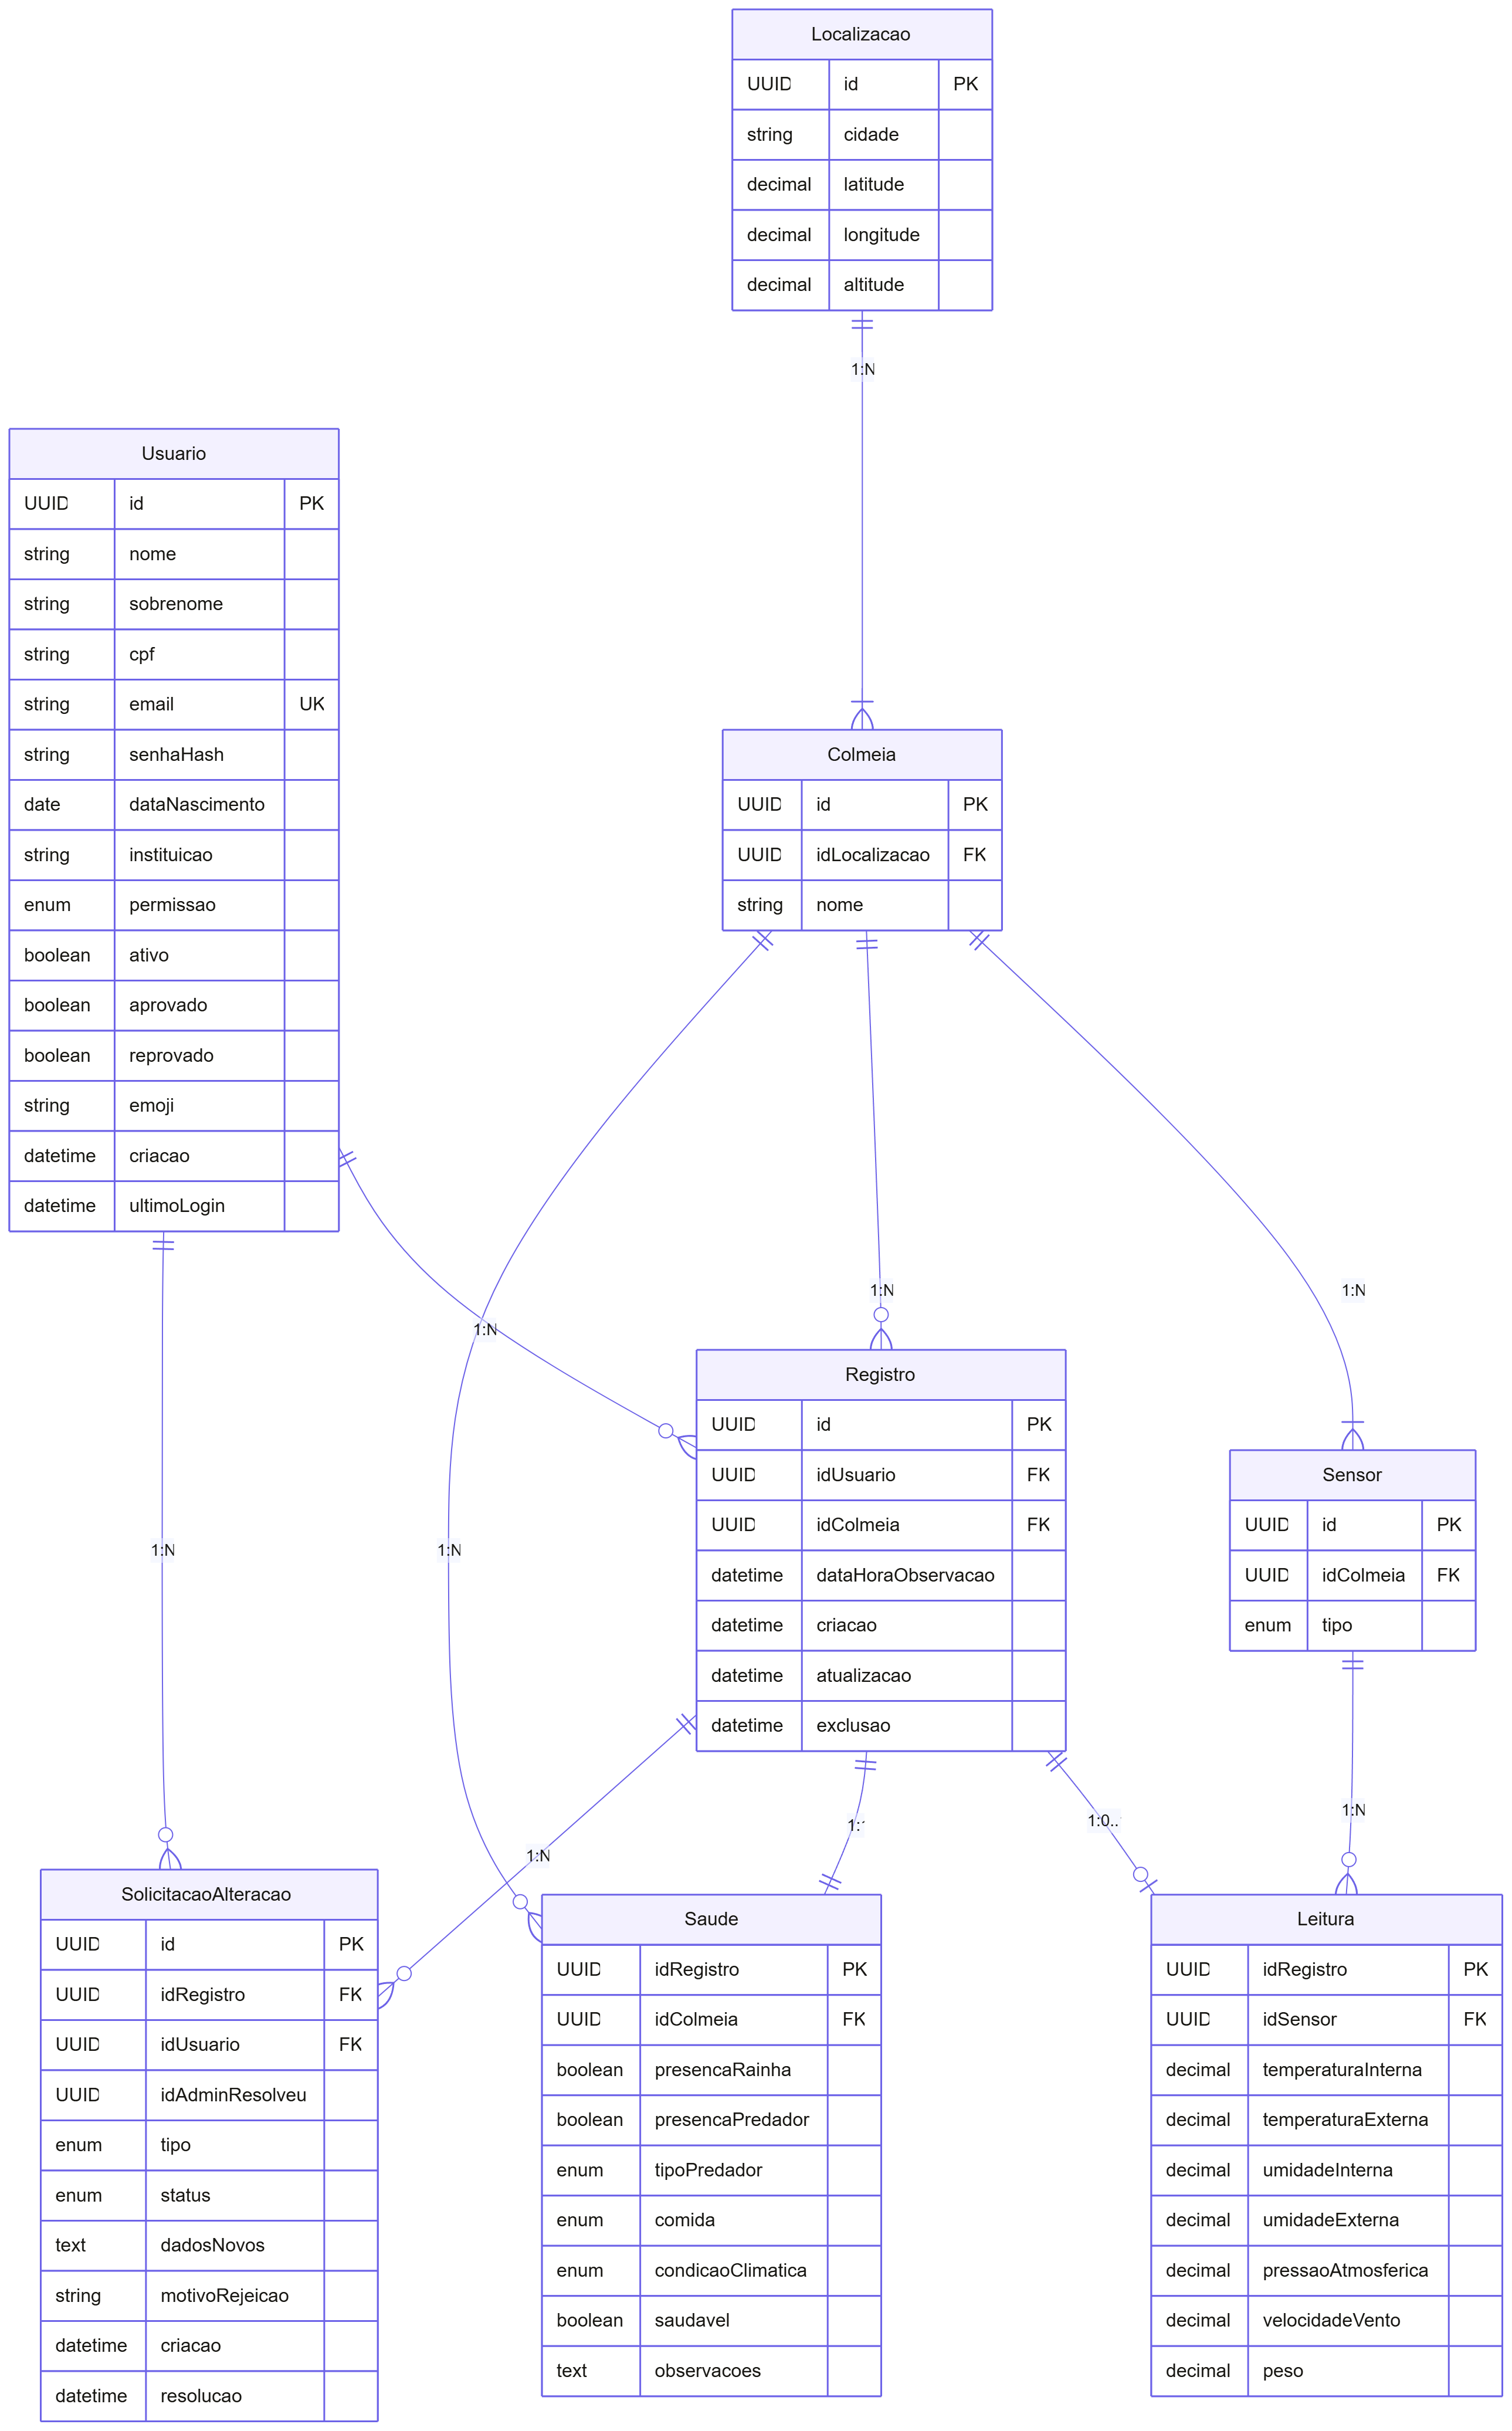
\includegraphics[width=0.5\textwidth, height=15cm]{imgs/diagrama_banco_mer.png}
     \caption{Diagrama entidade-relacionamento do banco de dados.}
     \label{fig:diagrama}
\end{figure}

A principal entidade do modelo é \textit{Registro}, responsável por representar o estado da colmeia. Cada registro está associado simultaneamente a um usuário, responsável pelo lançamento das informações e a uma colmeia monitorada. Além da data e horário da observação, são armazenadas as datas de criação, atualização e exclusão do registro.

A exclusão de registros foi implementada por meio da técnica de \textit{soft delete}. Nessa abordagem, os registros não são removidos fisicamente do banco de dados, sendo apenas preenchido o campo correspondente à data de exclusão, permitindo que as informações permaneçam armazenadas para fins de auditoria e rastreabilidade. Desse modo, consultas realizadas pelo sistema retornam apenas registros ativos, enquanto os registros excluídos permanecem preservados para eventual recuperação ou verificação histórica \cite{fowlerapp2002}.

Cada registro possui duas entidades associadas: \textit{Saude} e \textit{Leitura}. A tabela \textit{Saude} armazena as informações obtidas durante a inspeção visual da colmeia, incluindo a presença da rainha, a ocorrência de predadores, o tipo de predador identificado, a disponibilidade de alimento, a condição climática observada, a avaliação geral da saúde da colônia e observações complementares registradas pelo pesquisador.

A tabela \textit{Leitura} armazena as variáveis ambientais coletadas durante a inspeção, composta por: temperatura interna e externa, umidade interna e externa, pressão atmosférica, velocidade do vento e peso da colmeia. Todos esses campos são opcionais, permitindo que uma inspeção seja registrada mesmo quando não houver medições disponíveis. Somente registros que possuem ao menos uma variável ambiental preenchida possuem uma entidade correspondente na tabela \textit{Leitura}.

A separação entre as tabelas \textit{Saude} e \textit{Leitura} foi adotada visando à evolução futura do sistema. Embora as medições sejam atualmente registradas manualmente pelos pesquisadores, o projeto prevê a integração com sensores instalados nas colmeias. Dessa forma, as informações ambientais poderão futuramente ser inseridas automaticamente, sem necessidade de alterações na estrutura do banco de dados.

As tabelas \textit{Colmeia} e \textit{Localizacao} armazenam as informações referentes aos apiários monitorados. Cada colmeia possui um nome identificador e está associada a uma localização, que registra a cidade, latitude, longitude e altitude. Uma mesma localização pode estar vinculada a diversas colmeias, caracterizando um relacionamento de um para muitos.

Cada colmeia também pode possuir um ou mais sensores cadastrados na tabela \textit{Sensor}, responsável por identificar os equipamentos instalados e o tipo de medição realizada por cada dispositivo. Embora as leituras ainda sejam inseridas manualmente, esse relacionamento foi mantido para permitir a futura associação entre sensores físicos e os dados registrados pelo sistema.

A tabela \textit{Usuario} concentra as informações cadastrais dos pesquisadores e administradores. O endereço de e-mail possui restrição de unicidade, enquanto o Cadastro de Pessoa Física (CPF) possui apenas um índice para otimizar consultas, permitindo que um pesquisador realize novo cadastro utilizando outro endereço de e-mail caso sua conta anterior seja desativada.

O processo de aprovação de novos usuários é controlado pelos campos \textit{ativo}, \textit{aprovado} e \textit{reprovado}. Após a realização do cadastro, o usuário permanece ativo, porém sem autorização para acessar o sistema até que sua solicitação seja analisada por um administrador. Em caso de aprovação, o acesso é liberado. Caso a solicitação seja rejeitada, o usuário permanece impedido de utilizar as funcionalidades restritas da aplicação. O nível de acesso é definido pelo campo \textit{permissao}, que diferencia pesquisadores e administradores.

As solicitações de modificação dos registros são armazenadas na tabela \textit{SolicitacaoAlteracao}. Pesquisadores não possuem permissão para alterar diretamente os dados já registrados, de modo que qualquer solicitação de edição ou exclusão gera um novo registro nessa tabela, contendo o tipo da solicitação, seu estado atual e o usuário responsável pela requisição.

Nas solicitações de edição, os novos valores propostos são armazenados no campo \textit{dadosNovos} em formato \textit{JSON}. Enquanto a solicitação permanece pendente, nenhuma alteração é realizada sobre o registro original. Após a aprovação pelo administrador, o \textit{backend} interpreta essas informações e atualiza o registro correspondente. Essa estratégia preserva o histórico das informações e permite rastrear todas as alterações realizadas ao longo da utilização do sistema.

\subsection{Backend}

O \textit{backend} é responsável por validar as operações realizadas pelos usuários antes que qualquer alteração seja realizada no banco de dados. Entre essas validações estão a verificação das permissões de acesso, a consistência dos dados recebidos e a aplicação das regras de negócio definidas para cada funcionalidade do sistema. Implementadas em arquitetura monolítica, as funcionalidades foram organizadas em \textit{controllers}, cada um responsável por um conjunto específico de operações, facilitando a organização do código, manutenção e implementação de novas funcionalidades.

Entre as principais regras de negócio validadas, destacam-se a unicidade do endereço de e-mail e a verificação do CPF no cadastro de usuários, o armazenamento da senha de forma cifrada e a liberação do acesso apenas para contas ativas e previamente aprovadas por um administrador. 
O processo de aprovação impede que um administrador desative, reprove ou altere a própria permissão, evitando o bloqueio acidental do sistema. Quanto aos registros, apenas pesquisadores aprovados podem criar novas observações, e a associação de variáveis ambientais à tabela \textit{Leitura} ocorre somente quando há medições informadas e um sensor cadastrado para a colmeia. A exclusão de registros e de colmeias é tratada por meio de \textit{soft delete}, preservando as informações armazenadas. Além disso, pesquisadores não alteram registros diretamente, de modo que qualquer solicitação de edição ou exclusão permanece pendente até a aprovação de um administrador, não sendo permitida mais de uma solicitação pendente do mesmo tipo para um mesmo registro. Essas regras foram verificadas pelos testes automatizados descritos na metodologia.

A Tabela \ref{tab:endpoints} apresenta os endpoints implementados na aplicação, organizados por \textit{controller}, indicando o método \textit{HTTP} utilizado, a rota correspondente e o nível de acesso exigido para cada operação.

\renewcommand{\arraystretch}{1.0}

\begin{longtable}{llp{5cm}l}
\caption{Endpoints da API REST.}
\label{tab:endpoints}\\

\hline
\textbf{Método} & \textbf{Rota} & \textbf{Descrição} & \textbf{Acesso} \\
\hline
\multicolumn{4}{l}{\textit{AuthController}} \\
\hline
POST & /api/auth/register & Cadastro de usuários & Público \\
POST & /api/auth/login    & Autenticação e geração de token & Público \\
\hline
\multicolumn{4}{l}{\textit{PublicoController}} \\
\hline
GET & /api/publico/registros & Listagem de registros com filtros & Público \\
GET & /api/publico/colmeias  & Listagem de colmeias & Público \\
GET & /api/publico/periodo   & Período de registros disponíveis & Público \\
\hline
\multicolumn{4}{l}{\textit{ColmeiasController}} \\
\hline
GET & /api/colmeias & Listagem de colmeias para seleção no formulário & Autenticado \\
\hline
\multicolumn{4}{l}{\textit{RegistrosController}} \\
\hline
POST   & /api/registros      & Criação de registro de observação & Autenticado \\
GET    & /api/registros      & Listagem dos 50 registros mais recentes & Autenticado \\
PUT    & /api/registros/\{id\} & Edição de registros & Autenticado \\
DELETE & /api/registros/\{id\} & Exclusão de registros & Autenticado \\
\hline
\multicolumn{4}{l}{\textit{PerfilController}} \\
\hline
GET & /api/perfil & Listagem perfil usuário & Autenticado \\
PUT & /api/perfil & Atualização perfil usuário & Autenticado \\
\hline
\multicolumn{4}{l}{\textit{AdminController}} \\
\hline
GET   & /api/admin/usuarios                        & Listagem de usuários & Admin \\
PATCH & /api/admin/usuarios/\{id\}/aprovar          & Aprovação de cadastro & Admin \\
PATCH & /api/admin/usuarios/\{id\}/reprovar         & Reprovação de cadastro & Admin \\
PATCH & /api/admin/usuarios/\{id\}/desativar        & Desativação de usuário & Admin \\
PATCH & /api/admin/usuarios/\{id\}/permissao        & Alteração de permissão & Admin \\
GET   & /api/admin/colmeias                        & Listagem de colmeias & Admin \\
POST  & /api/admin/colmeias                        & Cadastro de colmeia & Admin \\
PUT   & /api/admin/colmeias/\{id\}                  & Edição de colmeia & Admin \\
PATCH & /api/admin/colmeias/\{id\}/desativar        & Desativação de colmeia & Admin \\
PATCH & /api/admin/colmeias/\{id\}/reativar         & Reativação de colmeia & Admin \\
GET   & /api/admin/solicitacoes                    & Listagem de solicitações de alteração & Admin \\
POST  & /api/admin/solicitacoes/\{id\}/aprovar      & Aprovação de solicitação & Admin \\
POST  & /api/admin/solicitacoes/\{id\}/rejeitar     & Rejeição de solicitação & Admin \\
\hline
\end{longtable}

\subsection{Frontend}

A aplicação foi organizada em páginas associadas a rotas, seguindo a convenção baseada no sistema de arquivos do \textit{Next.js}. Os elementos compartilhados entre as diferentes telas foram implementados como componentes reutilizáveis, reduzindo a duplicação de código e aumentando a centralização.

O controle de autenticação é realizado por meio de um \textit{token JWT} obtido durante o processo de \textit{login}. Após a autenticação com e-mail e senha, o \textit{token} é armazenado no navegador e enviado automaticamente em todas as requisições destinadas aos serviços protegidos da \textit{API}. As páginas restritas verificam a existência de uma sessão válida antes de serem carregadas, impedindo o acesso de usuários não autenticados.

A Tabela~\ref{tab:paginas} apresenta as páginas implementadas na aplicação, indicando a rota correspondente, a finalidade de cada uma e o nível de acesso exigido.

\renewcommand{\arraystretch}{1.0}

\begin{longtable}{lp{5cm}l}
\caption{Páginas da aplicação.}
\label{tab:paginas}\\

\hline
\textbf{Rota} & \textbf{Descrição} & \textbf{Acesso} \\
\hline
/ & Página de apresentação do projeto & Público \\
/dados & Consulta, visualização e exportação dos registros & Público \\
/login & Autenticação no sistema & Público \\
/register & Cadastro de novo usuário & Público \\
/registro & Formulário para registro de observações & Autenticado \\
/perfil & Atualização dos dados cadastrais & Autenticado \\
/admin/usuarios & Gerenciamento de usuários & Admin \\
/admin/colmeias & Gerenciamento de colmeias & Admin \\
/admin/solicitacoes & Gerenciamento de solicitações de alteração & Admin \\
\hline
\end{longtable}

As páginas públicas e administrativas seguem um padrão visual comum, baseado em tabelas paginadas, formulários e componentes de filtragem. Para a visualização dos registros também foram implementados gráficos e ferramentas de exportação dos dados para \texttt{.csv}, permitindo diferentes formas de exploração das informações armazenadas.

\section{Resultados e Discussões}

A implantação da arquitetura proposta resultou em uma plataforma \textit{web} funcional e acessível publicamente, disponível no endereço \url{http://colmeiamelipona.duckdns.org}. As interfaces desenvolvidas implementam as regras de negócio e os fluxos de acesso definidos na metodologia, viabilizando a interação dos diferentes perfis de usuários com o banco de dados de forma intuitiva e padronizada.

A \textit{Homepage} tem como objetivo a disseminação das informações e a apresentação do projeto 

\begin{figure}[H]
     \centering
     \includegraphics[width=1\textwidth, height=8cm]{imgs/home.png}
     \caption{Captura de tela da Homepage}
     \label{fig:home1}
\end{figure}

\begin{figure}[H]
     \centering
     \includegraphics[width=1\textwidth, height=8cm]{imgs/home2.png}
     \caption{Captura de tela da Homepage}
     \label{fig:home2}
\end{figure}

A página de consulta pública dos dados, apresentada na Figura \ref{fig:dados}, disponibiliza filtragem por colmeia e por período, delimitado automaticamente entre a data do primeiro e a do último registro disponíveis. 

\begin{figure}[H]
     \centering
     \includegraphics[width=1\textwidth, height=8cm]{imgs/dados.png}
     \caption{Captura de tela da página de dados pública}
     \label{fig:dados}
\end{figure}

Para o cadastro de novos usuários são aplicadas validações sobre os dados informados, exigindo nome e sobrenome com ao menos três caracteres, CPF válido, vínculo com uma instituição que possua ao menos uma colmeia cadastrada, idade mínima de 14 anos e senha com pelo menos seis caracteres. O endereço de e-mail é único, enquanto o CPF pode se repetir, uma vez que não há mecanismo de recuperação de senha, permitindo novo cadastro em caso de desativação da conta anterior.
O acesso às áreas restritas do sistema só pode ser realizado após aprovação do cadastro por um administrador.

\begin{figure}[H]
     \centering
     \includegraphics[width=1\textwidth, height=8cm]{imgs/cadastro.png}
     \caption{Captura de tela da página de cadastro}
     \label{fig:cadastro}
\end{figure}

\begin{figure}[H]
     \centering
     \includegraphics[width=1\textwidth, height=8cm]{imgs/login.png}
     \caption{Captura de tela da página de login}
     \label{fig:login}
\end{figure}

Após a autenticação, os usuários podem registrar o estado de saúde da colmeia por meio de um formulário. A data e o horário da observação são obtidos automaticamente a partir do dispositivo utilizado, embora permitam edição manual e os campos referentes aos dados vindos dos sensores aceitam apenas valores numéricos. Quando registrada a presença de um predador não incluso entre as opções predefinidas, é disponibilizado um campo para especificação manual.

\begin{figure}[H]
     \centering
     \includegraphics[width=1\textwidth, height=8cm]{imgs/registro1.png}
     \caption{Captura de tela da página de registro do estado de saúde da colmeia}
     \label{fig:registro1}
\end{figure}

\begin{figure}[H]
     \centering
     \includegraphics[width=1\textwidth, height=8cm]{imgs/registro2.png}
     \caption{Captura de tela da página de registro do estado de saúde da colmeia}
     \label{fig:registro2}
\end{figure}

A visualização dos dados apresenta recursos distintos conforme o perfil do usuário. O administrador pode editar e excluir registros diretamente, conforme a Figura \ref{fig:dados_login}. O pesquisador, por sua vez, pode solicitar a edição ou a exclusão de um registro, submetendo a alteração à aprovação de um administrador.

\begin{figure}[H]
     \centering
     \includegraphics[width=1\textwidth, height=8cm]{imgs/dados_login.png}
     \caption{Captura de tela da página de dados após login como administrador(a)}
     \label{fig:dados_login}
\end{figure}

\begin{figure}[H]
     \centering
     \includegraphics[width=1\textwidth, height=8cm]{imgs/dados_editar_pesquisador.png}
     \caption{Captura de tela da página de dados após login como pesquisador(a)}
     \label{fig:dados_login_pesquisador}
\end{figure}

\begin{figure}[H]
     \centering
     \includegraphics[width=1\textwidth, height=8cm]{imgs/editar_dados.png}
     \caption{Captura de tela da página de dados durante solicitação de alteração de registro}
     \label{fig:dados_login_alterando}
\end{figure}

\begin{figure}[H]
     \centering
     \includegraphics[width=1\textwidth, height=8cm]{imgs/dados_editado_pesquisador.png}
     \caption{Captura de tela da página de dados após solicitação de alteração de registro}
     \label{fig:dados_login_alterado}
\end{figure}

\begin{figure}[H]
     \centering
     \includegraphics[width=1\textwidth, height=8cm]{imgs/dados_excluir_pesquisador.png}
     \caption{Captura de tela da página de dados após solicitação de exclusão}
     \label{fig:dados_login_excluido}
\end{figure}

A aba de \textit{Dashboard} permite o acompanhamento da evolução dos registros ao longo do tempo, enquanto a de Correlação possibilita a análise da relação entre duas variáveis do registro.

\begin{figure}[H]
     \centering
     \includegraphics[width=1\textwidth, height=8cm]{imgs/dashboard1.png}
     \caption{Captura de tela da página de dados na aba Dashboard}
     \label{fig:dashboard1}
\end{figure}

\begin{figure}[H]
     \centering
     \includegraphics[width=1\textwidth, height=8cm]{imgs/dashboard2.png}
     \caption{Captura de tela da página de dados na aba Dashboard}
     \label{fig:dashboard2}
\end{figure}

\begin{figure}[H]
     \centering
     \includegraphics[width=1\textwidth, height=8cm]{imgs/dashboard3.png}
     \caption{Captura de tela da página de dados na aba Dashboard}
     \label{fig:dashboard3}
\end{figure}

\begin{figure}[H]
     \centering
     \includegraphics[width=1\textwidth, height=8cm]{imgs/correlacao.png}
     \caption{Captura de tela da página de visualização da correlação}
     \label{fig:correlacao}
\end{figure}

As funcionalidades administrativas contemplam a gestão de usuários, de colmeias e das solicitações de alteração. A página de gestão de usuários organiza as solicitações de cadastro e usuários ativos, permitindo distinguir os cadastros pendentes, aprovados, rejeitados e desativados.

\begin{figure}[H]
     \centering
     \includegraphics[width=1\textwidth, height=8cm]{imgs/usuarios_todos.png}
     \caption{Captura de tela da página de gestão de usuários na aba todos}
     \label{fig:usuarios_todo}
\end{figure}

\begin{figure}[H]
     \centering
     \includegraphics[width=1\textwidth, height=8cm]{imgs/usuarios_aprovados.png}
     \caption{Captura de tela da página de gestão de usuários na aba aprovados}
     \label{fig:usuarios_aprovados}
\end{figure}

A página de gestão de colmeias reúne o cadastro e a administração das colmeias monitoradas.

\begin{figure}[H]
     \centering
     \includegraphics[width=1\textwidth, height=8cm]{imgs/colmeias.png}
     \caption{Captura de tela da página de gestão de colmeias}
     \label{fig:colmeias}
\end{figure}

A gestão das solicitações de alteração, ilustrada nas Figuras \ref{fig:aprovacoes_pendentes} a \ref{fig:aprovacoes_rejeitadas}, permite comparar o registro atual e a alteração proposta, além de registrar uma justificativa para a aprovação ou a rejeição de cada solicitação, se necessário.


\begin{figure}[H]
     \centering
     \includegraphics[width=1\textwidth, height=8cm]{imgs/solicitacao_banco.png}
     \caption{Captura de tela da página de gestão de solicitações pendentes}
     \label{fig:aprovacoes_pendentes}
\end{figure}

\begin{figure}[H]
     \centering
     \includegraphics[width=1\textwidth, height=8cm]{imgs/alteracoes_aprovadas.png}
     \caption{Captura de tela da página de gestão de solicitações aprovadas}
     \label{fig:alteracoes_aprovadas}
\end{figure}

\begin{figure}[H]
     \centering
     \includegraphics[width=1\textwidth, height=8cm]{imgs/alteracoes_rejeitadas.png}
     \caption{Captura de tela da página de gestão de solicitações rejeitadas}
     \label{fig:aprovacoes_rejeitadas}
\end{figure}

Ao selecionar o ícone de perfil, o usuário visualiza o ícone escolhido, o primeiro nome, o e-mail e o nível de permissão, além das opções para editar o perfil e encerrar a sessão.

\begin{figure}[H]
     \centering
     \includegraphics[width=1\textwidth, height=8cm]{imgs/clique_login.png}
     \caption{Captura de tela quando ícone de perfil é clicado}
     \label{fig:icone_perfil}
\end{figure}

Na edição de perfil, todas as informações cadastrais podem ser atualizadas, com exceção do CPF e do nível de acesso, este último modificável apenas por um administrador.

\begin{figure}[H]
     \centering
     \includegraphics[width=1\textwidth, height=8cm]{imgs/editar_usuario.png}
     \caption{Captura de tela da página de edição do perfil}
     \label{fig:perfil}
\end{figure}

O usuário pode selecionar o ícone para o seu perfil entre as opções compostas pela biblioteca \textit{Lucide}.

\begin{figure}[H]
     \centering
     \includegraphics[width=1\textwidth, height=8cm]{imgs/icone_perfil.png}
     \caption{Captura de tela da página de edição do perfil após clicar em editar ícone}
     \label{fig:editar_icone}
\end{figure}

Além da interface, as operações da \textit{API} podem ser testadas de forma autenticada por meio da documentação gerada pelo \textit{Swagger}.

\begin{figure}[H]
     \centering
     \includegraphics[width=1\textwidth, height=8cm]{imgs/swagger1.png}
     \caption{Captura de tela dos endpoints no \textit{Swagger}}
     \label{fig:swagger}
\end{figure}

Ademais, os dados armazenados podem ser consultados diretamente pelos \textit{endpoints} públicos da \textit{API}, sem necessidade de autenticação, o que amplia as possibilidades de reutilização por outros sistemas e ferramentas de análise. O sistema encontra-se disponível no endereço \url{http://colmeiamelipona.duckdns.org}, e os dados públicos podem ser acessados a partir de \url{http://colmeiamelipona.duckdns.org/api/publico/}.

\begin{figure}[H]
     \centering
     \includegraphics[width=1\textwidth, height=8cm]{imgs/api.png}
     \caption{Captura de tela quando \textit{API} é acessada}
     \label{fig:api}
\end{figure}

\subsection{Discussão}

A integração entre fatores ambientais e sanitários amplia o potencial de utilização dos registros produzidos ao longo do tempo. Torna-se mais difícil identificar quais fatores estão associados ao enfraquecimento das colônias e quais combinações de estressores causam maior impacto sobre sua saúde quando os dados são registrados em momentos distintos ou de forma não padronizada \cite{brydenstress2013}.

As informações ambientais são inseridas manualmente pelos pesquisadores, tornando a frequência e a quantidade de registros dependentes da realização das inspeções. Tal característica pode reduzir a granularidade temporal dos dados quando comparada a sistemas baseados em monitoramento automatizado por sensores. Entretanto, a estrutura do banco de dados foi projetada considerando essa evolução, permitindo a futura integração de dispositivos capazes de realizar medições contínuas sem necessidade de alterações significativas na modelagem.

Atualmente, a interface permite a visualização de gráficos de correlação relacionando apenas duas variáveis por vez, o que restringe a exploração simultânea de múltiplos estressores. Considerando que o declínio das colônias geralmente resulta da interação entre diversos estressores, a incorporação de análises multivariadas e ferramentas estatísticas mais avançadas poderá ampliar o potencial analítico da plataforma em trabalhos futuros.

Portanto, a principal contribuição do sistema desenvolvido consiste na centralização de registros em um banco de dados estruturado com mecanismos de controle de acesso e gerenciamento de usuários administradores. Diferentes iniciativas já demonstraram a importância do monitoramento de colônias por meio da coleta de variáveis ambientais ou indicadores de saúde, contribuindo para o avanço das pesquisas relacionadas à conservação de abelhas. A estrutura proposta neste trabalho busca complementar essas abordagens ao permitir o registro integrado dessas informações, reduzindo a fragmentação dos dados e favorecendo análises históricas.

\section{Conclusão}
A disponibilidade de registros padronizados representa um dos principais desafios para estudos que buscam compreender a influência de fatores ambientais sobre a saúde de colônias de \textit{Melipona quadrifasciata}. Nesse contexto, o sistema proposto estabelece uma base para o armazenamento e a organização dessas informações, permitindo que os dados produzidos durante o monitoramento sejam utilizados em estudos futuros.

Embora o sistema tenha sido desenvolvido para atender às necessidades atuais de registro e gerenciamento dos dados, sua estrutura possibilita a incorporação de novas funcionalidades sem alterações significativas na organização das informações armazenadas. Ademais, o modelo implementado fornece uma estrutura adequada para análises estatísticas, mineração de dados e aprendizado de máquina futuros. Com a evolução do conjunto de registros, torna-se possível investigar relações entre condições ambientais e alterações no estado das colônias, contribuindo para a compreensão dos fatores associados ao seu enfraquecimento e apoiando estratégias preventivas de manejo e conservação.

\section*{Agradecimentos}
Agradeço a todos que colocaram sua pedra para formar o caminho ladrilhado colorido que hoje percorro.

Em especial a minha família, professores e amigos, a paciência e incentivo de vocês todo o dia muda um pouco do mundo.

\bibliography{referencias}

\end{document}